% !TEX TS-program = pdflatex
\documentclass[11pt]{article}

% -------------------- Packages --------------------
\usepackage[a4paper,margin=1in]{geometry}
\usepackage{amsmath,amssymb}
\usepackage[T1]{fontenc}
\usepackage{lmodern}
\usepackage{xcolor}
\usepackage{tcolorbox}
\tcbuselibrary{skins,breakable}
\usepackage{enumitem}
\usepackage{hyperref}
\usepackage{tikz}
\usetikzlibrary{calc,angles,quotes,positioning}

\pagestyle{empty}

% -------------------- Dark Theme Colors --------------------
\definecolor{bg}{HTML}{000000}
\definecolor{pairbg}{HTML}{121212}
\definecolor{solbg}{HTML}{0A0A0A}
\definecolor{border}{HTML}{2A2A2A}
\definecolor{text}{HTML}{FFFFFF}
\definecolor{muted}{HTML}{C9CDD3}
\definecolor{gold}{HTML}{FFD700}
\definecolor{green}{HTML}{4ADE80}
\definecolor{cyan}{HTML}{38BDF8}

\pagecolor{bg}
\color{text}

\hypersetup{
  colorlinks=true,
  linkcolor=cyan,
  urlcolor=cyan
}

\setlength{\parindent}{0pt}
\setlength{\parskip}{10pt}

\setlist[itemize]{left=1.4em,itemsep=6pt,topsep=6pt}
\setlist[enumerate]{left=1.6em,itemsep=4pt,topsep=4pt}

% -------------------- tcolorbox Base --------------------
\tcbset{
  enhanced,
  breakable,
  arc=12pt,
  boxrule=0.8pt,
  left=16pt,right=16pt,top=12pt,bottom=12pt
}

\newtcolorbox{QAPair}[1]{%
  colback=pairbg,
  colbacklower=solbg,
  colframe=border,
  coltext=text,
  title=\textcolor{gold}{\bfseries #1},
  fonttitle=\bfseries,
  coltitle=text,
  segmentation style={draw=border, dashed, line width=0.6pt},
}

\newtcolorbox{QuickBox}{%
  colback=pairbg,
  colframe=cyan,
  coltext=text,
  fontupper=\color{text},
  borderline north={4pt}{0pt}{cyan},
  arc=14pt,
  boxrule=0.8pt
}

% Helper for step headings
\newcommand{\Step}[1]{\textcolor{muted}{\textbf{Step #1:}}}

% -------------------- Internal angle (ALWAYS) helper --------------------
% This picks the < 180° (interior) angle automatically (prevents drawing 360°-x reflex angles).
\tikzset{
  IntAngle/.style={
    draw=cyan, thick,
    fill=cyan!25, fill opacity=0.12,
    angle radius=8mm,
    angle eccentricity=1.25
  }
}

\newcommand{\InternalAngle}[5][]{%
  % #1 = tikz pic options (e.g. IntAngle)
  % #2 = first point, #3 = vertex, #4 = third point, #5 = label (can be empty)
  \pgfmathanglebetweenpoints{\pgfpointanchor{#3}{center}}{\pgfpointanchor{#2}{center}}
  \let\angA\pgfmathresult
  \pgfmathanglebetweenpoints{\pgfpointanchor{#3}{center}}{\pgfpointanchor{#4}{center}}
  \let\angC\pgfmathresult
  \pgfmathsetmacro{\delang}{Mod(\angC-\angA,360)}%
  \def\lbl{#5}%
  \ifdim \delang pt > 180pt
    \if\relax\detokenize{#5}\relax
      \pic[#1]{angle=#4--#3--#2};
    \else
      \pic[#1,"$\displaystyle #5$"]{angle=#4--#3--#2};
    \fi
  \else
    \if\relax\detokenize{#5}\relax
      \pic[#1]{angle=#2--#3--#4};
    \else
      \pic[#1,"$\displaystyle #5$"]{angle=#2--#3--#4};
    \fi
  \fi
}

% ============================================================
\begin{document}

\begin{center}
{\LARGE\bfseries \textcolor{gold}{Exercise 8.6 --- Solutions}}\\[-2pt]
\end{center}

\begin{QuickBox}
{\color{cyan}\bfseries Quick formulas (Trigonometry)}\par\medskip
\begin{itemize}
\item \textbf{Right triangle:} $\sin\theta=\dfrac{\text{opp}}{\text{hyp}}$, $\cos\theta=\dfrac{\text{adj}}{\text{hyp}}$, $\tan\theta=\dfrac{\text{opp}}{\text{adj}}$.
\item \textbf{Pythagoras:} $\text{hyp}^2=\text{opp}^2+\text{adj}^2$.
\item \textbf{Cosine rule:} $c^2=a^2+b^2-2ab\cos C$.
\item \textbf{Sine rule:} $\dfrac{a}{\sin A}=\dfrac{b}{\sin B}=\dfrac{c}{\sin C}$.
\item \textbf{Angle between a line and a plane:} equals the angle between the line and its \emph{projection} on the plane.
\end{itemize}

\medskip
{\color{cyan}\bfseries Quick diagrams (one per concept)}\par\smallskip

% --- Right triangle diagram
\begin{center}
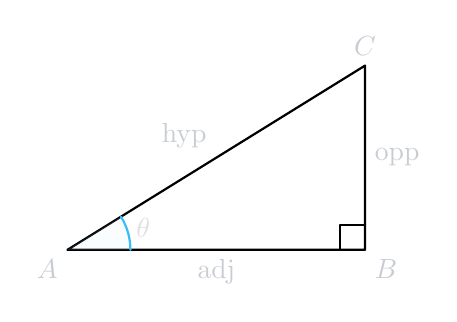
\begin{tikzpicture}[scale=0.9, line cap=round, line join=round]
  \coordinate (A) at (0,0);
  \coordinate (B) at (4.2,0);
  \coordinate (C) at (4.2,2.6);

  \draw[thick] (A)--(B)--(C)--cycle;
  % right angle marker at B
  \draw[thick] ($(B)+(-0.35,0)$)--($(B)+(-0.35,0.35)$)--($(B)+(0,0.35)$);

  \node[below] at ($(A)!0.5!(B)$) {\textcolor{muted}{adj}};
  \node[right] at ($(B)!0.5!(C)$) {\textcolor{muted}{opp}};
  \node[above left] at ($(A)!0.5!(C)$) {\textcolor{muted}{hyp}};

  \InternalAngle[IntAngle]{B}{A}{C}{\theta}
  \node[below left] at (A) {\textcolor{muted}{$A$}};
  \node[below right] at (B) {\textcolor{muted}{$B$}};
  \node[above] at (C) {\textcolor{muted}{$C$}};
\end{tikzpicture}
\end{center}

% --- Sine/Cosine rule triangle diagram
\begin{center}
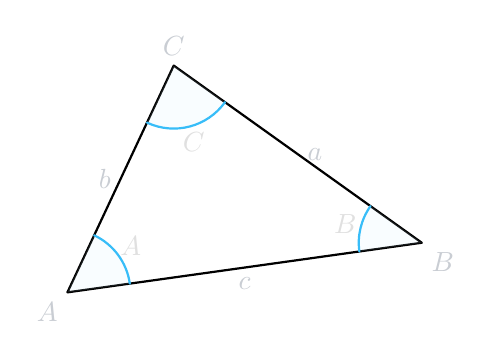
\begin{tikzpicture}[scale=0.9, line cap=round, line join=round]
  \coordinate (A) at (0,0);
  \coordinate (B) at (5.0,0.7);
  \coordinate (C) at (1.5,3.2);

  \draw[thick] (A)--(B)--(C)--cycle;

  \node[below left] at (A) {\textcolor{muted}{$A$}};
  \node[below right] at (B) {\textcolor{muted}{$B$}};
  \node[above] at (C) {\textcolor{muted}{$C$}};

  \node[below] at ($(A)!0.5!(B)$) {\textcolor{muted}{$c$}};
  \node[right] at ($(B)!0.5!(C)$) {\textcolor{muted}{$a$}};
  \node[left] at ($(A)!0.5!(C)$) {\textcolor{muted}{$b$}};

  \InternalAngle[IntAngle]{C}{A}{B}{A}
  \InternalAngle[IntAngle]{A}{B}{C}{B}
  \InternalAngle[IntAngle]{B}{C}{A}{C}
\end{tikzpicture}
\end{center}

% --- Line & plane projection diagram
\begin{center}
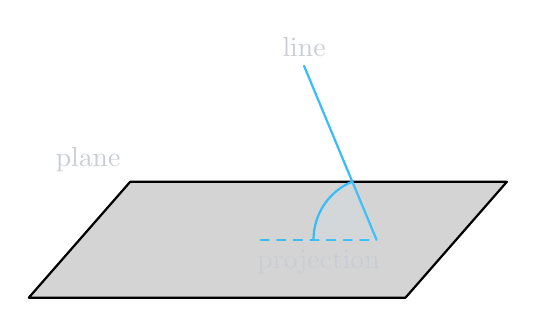
\begin{tikzpicture}[scale=0.92, line cap=round, line join=round]
  % plane as a parallelogram
  \coordinate (P1) at (0,0);
  \coordinate (P2) at (5.2,0);
  \coordinate (P3) at (6.6,1.6);
  \coordinate (P4) at (1.4,1.6);

  \fill[border, opacity=0.20] (P1)--(P2)--(P3)--(P4)--cycle;
  \draw[thick] (P1)--(P2)--(P3)--(P4)--cycle;

  \node[above left] at (P4) {\textcolor{muted}{plane}};

  % point above plane and projection
  \coordinate (X) at (3.8,3.2);
  \coordinate (Y) at (4.8,0.8); % point on plane (projection target)
  \coordinate (Z) at (3.2,0.8); % another point on plane for projection line

  % line in space
  \draw[cyan, thick] (X)--(Y);
  \node[above] at (X) {\textcolor{muted}{line}};

  % projection on plane
  \draw[cyan, thick, dashed] (Z)--(Y);
  \node[below] at ($(Z)!0.5!(Y)$) {\textcolor{muted}{projection}};

  % show the angle between line and its projection
  \InternalAngle[IntAngle]{Z}{Y}{X}{}
\end{tikzpicture}
\end{center}

\end{QuickBox}

% ============================================================
% Q1
\begin{QAPair}{Question 1}
\textcolor{gold}{\bfseries Question:} In the cuboid $ABCDEFGH$, calculate $CF$ (given $DC=24\text{ cm}$, $CG=8\text{ cm}$ and $\angle FHG=30^\circ$ as shown).\\[6pt]

\begin{center}
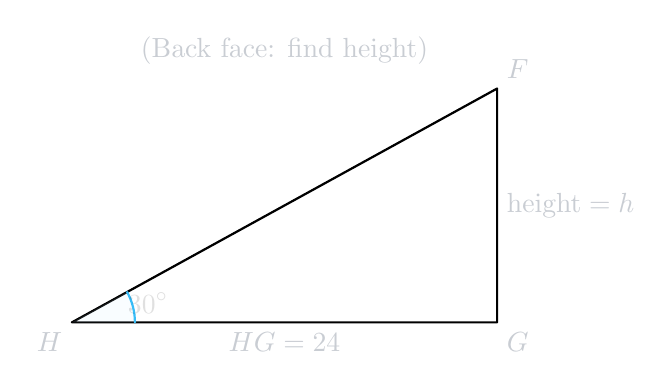
\begin{tikzpicture}[scale=0.9, line cap=round, line join=round]
  % Triangle in back face to get height
  \coordinate (H) at (0,0);
  \coordinate (G) at (6,0);
  \coordinate (F) at (6,3.3);
  \draw[thick] (H)--(G)--(F)--cycle;
  \draw[dashed] (H)--(F);

  % ALWAYS internal (non-reflex) angle
  \InternalAngle[IntAngle]{F}{H}{G}{30^\circ}

  \node[below] at ($(H)!0.5!(G)$) {\textcolor{muted}{$HG=24$}};
  \node[right] at ($(G)!0.5!(F)$) {\textcolor{muted}{$\text{height}=h$}};
  \node[above right] at (F) {\textcolor{muted}{$F$}};
  \node[below left] at (H) {\textcolor{muted}{$H$}};
  \node[below right] at (G) {\textcolor{muted}{$G$}};
  \node[above] at (3,3.5) {\textcolor{muted}{(Back face: find height)}};
\end{tikzpicture}
\end{center}

\begin{center}
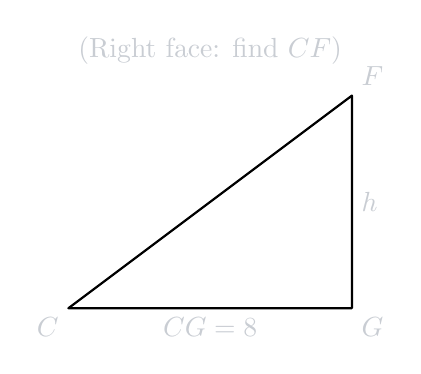
\begin{tikzpicture}[scale=0.9, line cap=round, line join=round]
  % Right face triangle to get CF
  \coordinate (C) at (0,0);
  \coordinate (G2) at (4,0);
  \coordinate (F2) at (4,3);
  \draw[thick] (C)--(G2)--(F2)--cycle;
  \draw[dashed] (C)--(F2);
  \node[below] at ($(C)!0.5!(G2)$) {\textcolor{muted}{$CG=8$}};
  \node[right] at ($(G2)!0.5!(F2)$) {\textcolor{muted}{$h$}};
  \node[above right] at (F2) {\textcolor{muted}{$F$}};
  \node[below left] at (C) {\textcolor{muted}{$C$}};
  \node[below right] at (G2) {\textcolor{muted}{$G$}};
  \node[above] at (2,3.3) {\textcolor{muted}{(Right face: find $CF$)}};
\end{tikzpicture}
\end{center}

\tcblower
\textcolor{green}{\bfseries Answer:}
\[
\begin{aligned}
\Step{1}\;& \text{In the back face }(HGF):\quad \tan 30^\circ=\frac{h}{HG}=\frac{h}{24}.\\
\Step{2}\;& h=24\tan 30^\circ=24\cdot\frac{1}{\sqrt{3}}=\frac{24}{\sqrt{3}}=8\sqrt{3}\ \text{cm}.\\
\Step{3}\;& \text{In the right face }(CFG):\quad CF^2=h^2+CG^2=(8\sqrt{3})^2+8^2.\\
\Step{4}\;& CF^2=192+64=256\;\Rightarrow\; CF=16\ \text{cm}.
\end{aligned}
\]
\end{QAPair}

% ============================================================
% Q2
\begin{QAPair}{Question 2}
\textcolor{gold}{\bfseries Question:} Find $\angle ACF$ in the given cuboid (dimensions $DC=12\text{ cm}$, $CG=10\text{ cm}$, $AD=9\text{ cm}$).\\[6pt]

\begin{center}
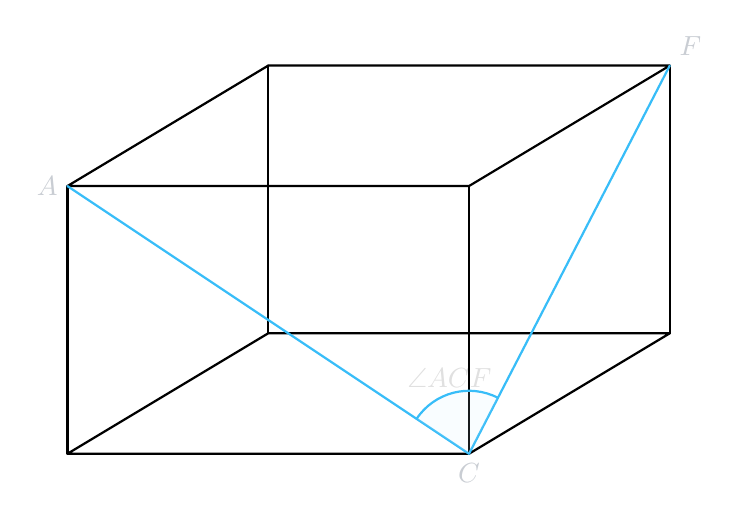
\begin{tikzpicture}[scale=0.85, line cap=round, line join=round]
  % simple cuboid projection
  \coordinate (D) at (0,0);
  \coordinate (C) at (6,0);
  \coordinate (G) at (9,1.8);
  \coordinate (H) at (3,1.8);

  \coordinate (A) at (0,4);
  \coordinate (B) at (6,4);
  \coordinate (F) at (9,5.8);
  \coordinate (E) at (3,5.8);

  % edges
  \draw[thick] (D)--(C)--(G)--(H)--cycle;
  \draw[thick] (A)--(B)--(F)--(E)--cycle;
  \draw[thick] (A)--(D);
  \draw[thick] (B)--(C);
  \draw[thick] (F)--(G);
  \draw[thick] (E)--(H);

  % diagonals for angle at C
  \draw[cyan, thick] (C)--(A);
  \draw[cyan, thick] (C)--(F);

  \node[left] at (A) {\textcolor{muted}{$A$}};
  \node[below] at (C) {\textcolor{muted}{$C$}};
  \node[above right] at (F) {\textcolor{muted}{$F$}};

  % ALWAYS internal (non-reflex) angle
  \InternalAngle[IntAngle]{A}{C}{F}{\angle ACF}
\end{tikzpicture}
\end{center}

\tcblower
\textcolor{green}{\bfseries Answer:}
\[
\begin{aligned}
\Step{1}\;& AC=\sqrt{12^2+9^2}=\sqrt{144+81}=15\ \text{cm}.\\
\Step{2}\;& CF=\sqrt{10^2+9^2}=\sqrt{100+81}=\sqrt{181}\ \text{cm}.\\
\Step{3}\;& AF=\sqrt{12^2+10^2}=\sqrt{144+100}=\sqrt{244}\ \text{cm}.\\
\Step{4}\;& \text{Use cosine rule in }\triangle ACF:\\
&\cos(\angle ACF)=\frac{AC^2+CF^2-AF^2}{2(AC)(CF)}
=\frac{225+181-244}{2(15)(\sqrt{181})}
=\frac{162}{30\sqrt{181}}.\\
\Step{5}\;& \angle ACF=\cos^{-1}\!\left(\frac{162}{30\sqrt{181}}\right)\approx 66.34^\circ.
\end{aligned}
\]
\end{QAPair}

% ============================================================
% Q3
\begin{QAPair}{Question 3}
\textcolor{gold}{\bfseries Question:} The perimeter of the square base of a pyramid is $36\text{ cm}$. Find (a) the diagonal of the base and (b) the height of the pyramid (given $\angle EAO=45^\circ$ as shown).\\[6pt]

\begin{center}
\begin{tikzpicture}[scale=0.95, line cap=round, line join=round]
  % base square (as a diamond for style)
  \coordinate (B) at (-3,0);
  \coordinate (C) at (0,-1.6);
  \coordinate (D) at (3,0);
  \coordinate (E) at (0,1.6);
  \coordinate (O) at (0,0);
  \coordinate (A) at (0,3.6);

  \draw[thick] (B)--(C)--(D)--(E)--cycle;
  \draw[dashed] (B)--(D);
  \draw[dashed] (C)--(E);
  \draw[cyan, thick] (A)--(O);
  \draw[cyan, thick] (A)--(E);
  \draw[dashed] (O)--(E);

  % ALWAYS internal (non-reflex) angle
  \InternalAngle[IntAngle]{E}{A}{O}{45^\circ}

  \node[above] at (A) {\textcolor{muted}{$A$}};
  \node[below] at (C) {\textcolor{muted}{$C$}};
  \node[left] at (B) {\textcolor{muted}{$B$}};
  \node[right] at (D) {\textcolor{muted}{$D$}};
  \node[above] at (E) {\textcolor{muted}{$E$}};
  \node[below right] at (O) {\textcolor{muted}{$O$}};
\end{tikzpicture}
\end{center}

\tcblower
\textcolor{green}{\bfseries Answer:}
\[
\begin{aligned}
\Step{1}\;& \text{Perimeter }=36\Rightarrow \text{side of square }s=\frac{36}{4}=9\ \text{cm}.\\
\Step{2}\;& \text{Diagonal of base}=s\sqrt{2}=9\sqrt{2}\ \text{cm}.\\
\Step{3}\;& OE=\frac{\text{diagonal}}{2}=\frac{9\sqrt{2}}{2}=\frac{9}{\sqrt{2}}\ \text{cm}.\\
\Step{4}\;& \text{In right }\triangle AOE\ (AO\perp\text{base}),\ \tan 45^\circ=\frac{OE}{AO}=1.\\
\Step{5}\;& \Rightarrow AO=OE=\frac{9}{\sqrt{2}}=\frac{9\sqrt{2}}{2}\approx 6.36\ \text{cm}.
\end{aligned}
\]
\[
\boxed{\text{Diagonal of base }=9\sqrt{2}\ \text{cm},\quad \text{Height }=AO=\frac{9\sqrt{2}}{2}\ \text{cm}.}
\]
\end{QAPair}

% ============================================================
% Q4
\begin{QAPair}{Question 4}
\textcolor{gold}{\bfseries Question:} The diagram shows a cylinder. Find the value of $\gamma$ in $\triangle ABC$ (given $AB=10\text{ cm}$, height $=30\text{ cm}$, and $\angle A=120^\circ$).\\[6pt]

\begin{center}
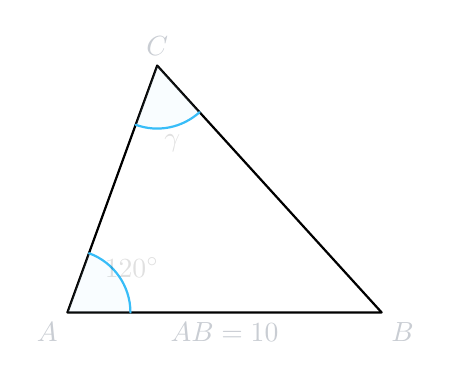
\begin{tikzpicture}[scale=0.95, line cap=round, line join=round]
  \coordinate (A) at (0,0);
  \coordinate (B) at (4.2,0);
  \coordinate (C) at (1.2,3.3);

  \draw[thick] (A)--(B)--(C)--cycle;

  % ALWAYS internal (non-reflex) angles
  \InternalAngle[IntAngle]{B}{A}{C}{120^\circ}
  \InternalAngle[IntAngle]{A}{C}{B}{\gamma}

  \node[below left] at (A) {\textcolor{muted}{$A$}};
  \node[below right] at (B) {\textcolor{muted}{$B$}};
  \node[above] at (C) {\textcolor{muted}{$C$}};
  \node[below] at ($(A)!0.5!(B)$) {\textcolor{muted}{$AB=10$}};
\end{tikzpicture}
\end{center}

\tcblower
\textcolor{green}{\bfseries Answer:}
\[
\begin{aligned}
\Step{1}\;& \text{Since }AB \text{ is the radius, }AB=10\text{ cm, and height }=30\text{ cm}.\\
\Step{2}\;& \text{Point }C\text{ is on the top rim, so }AC=\sqrt{10^2+30^2}=\sqrt{1000}=10\sqrt{10}\ \text{cm}.\\
\Step{3}\;& \text{Cosine rule in }\triangle ABC\text{ (angle at }A=120^\circ\text{):}\\
&BC^2=AB^2+AC^2-2(AB)(AC)\cos 120^\circ\\
&=10^2+(10\sqrt{10})^2-2(10)(10\sqrt{10})\left(-\frac12\right)
=100+1000+100\sqrt{10}.\\
\Step{4}\;& BC=\sqrt{1100+100\sqrt{10}}\approx 37.63\ \text{cm}.\\
\Step{5}\;& \text{Now use sine rule: }\ \frac{\sin\gamma}{AB}=\frac{\sin 120^\circ}{BC}\\
&\Rightarrow \sin\gamma=\frac{10\cdot \sin 120^\circ}{37.63}\approx \frac{10\cdot 0.8660}{37.63}\approx 0.2302.\\
\Step{6}\;& \gamma\approx \sin^{-1}(0.2302)\approx 13.30^\circ.
\end{aligned}
\]
\[
\boxed{\gamma \approx 13.3^\circ}
\]
\end{QAPair}

% ============================================================
% Q5
\begin{QAPair}{Question 5 (i) -- (iii)}
\textcolor{gold}{\bfseries Question:} In the cuboid (length $16\text{ cm}$, width $12\text{ cm}$, height $15\text{ cm}$), workers stand at $B$, $D$ and $H$.\\
(i) Find $BD$. \quad (ii) Find $BH$. \quad (iii) Find $\angle DBH$.\\[6pt]

\begin{center}
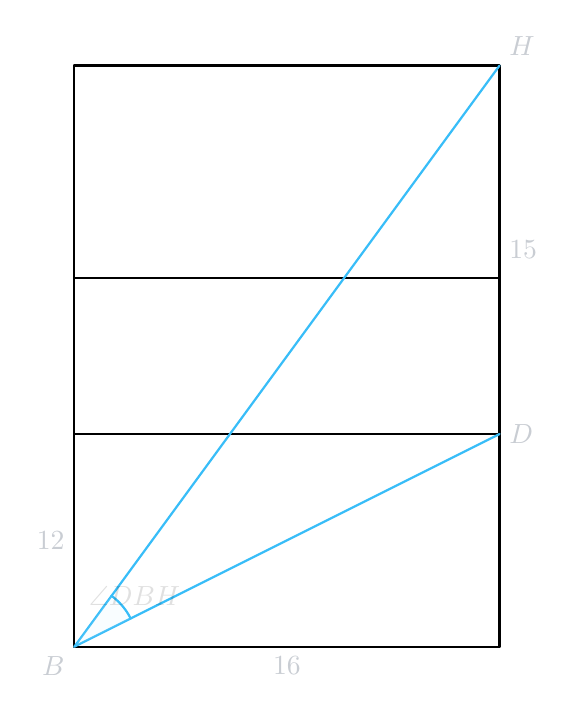
\begin{tikzpicture}[scale=0.9, line cap=round, line join=round]
  % base rectangle
  \coordinate (B) at (0,0);
  \coordinate (C) at (6,0);
  \coordinate (D) at (6,3);
  \coordinate (A) at (0,3);
  % top (shifted up)
  \coordinate (F) at (0,5.2);
  \coordinate (G) at (6,5.2);
  \coordinate (H) at (6,8.2);
  \coordinate (E) at (0,8.2);

  \draw[thick] (B)--(C)--(D)--(A)--cycle;
  \draw[thick] (F)--(G)--(H)--(E)--cycle;
  \draw[thick] (B)--(F);
  \draw[thick] (C)--(G);
  \draw[thick] (D)--(H);
  \draw[thick] (A)--(E);

  \draw[cyan, thick] (B)--(D);
  \draw[cyan, thick] (B)--(H);

  % ALWAYS internal (non-reflex) angle
  \InternalAngle[IntAngle]{D}{B}{H}{\angle DBH}

  \node[below left] at (B) {\textcolor{muted}{$B$}};
  \node[right] at (D) {\textcolor{muted}{$D$}};
  \node[above right] at (H) {\textcolor{muted}{$H$}};

  \node[below] at ($(B)!0.5!(C)$) {\textcolor{muted}{$16$}};
  \node[left] at ($(B)!0.5!(A)$) {\textcolor{muted}{$12$}};
  \node[right] at ($(D)!0.5!(H)$) {\textcolor{muted}{$15$}};
\end{tikzpicture}
\end{center}

\tcblower
\textcolor{green}{\bfseries Answer:}
\[
\begin{aligned}
\Step{1}\;& \text{On the base rectangle: }BD=\sqrt{16^2+12^2}=\sqrt{256+144}=\sqrt{400}=20\ \text{cm}.\\
\Step{2}\;& \text{In right }\triangle BDH\ (DH\perp \text{base}),\quad BH=\sqrt{BD^2+DH^2}=\sqrt{20^2+15^2}\\
&=\sqrt{400+225}=\sqrt{625}=25\ \text{cm}.\\
\Step{3}\;& \cos(\angle DBH)=\frac{BD}{BH}=\frac{20}{25}=0.8\\
&\Rightarrow \angle DBH=\cos^{-1}(0.8)\approx 36.87^\circ.
\end{aligned}
\]
\[
\boxed{BD=20\text{ cm},\quad BH=25\text{ cm},\quad \angle DBH\approx 36.87^\circ.}
\]
\end{QAPair}

% ============================================================
% Q6
\begin{QAPair}{Question 6}
\textcolor{gold}{\bfseries Question:} $O$ is the centre of the square-based pyramid $ABCDE$. Calculate the angle between side $AB$ and plane $BCDE$ if $AO=6\text{ cm}$ and the base side is $4\text{ cm}$ (as shown).\\[6pt]

\begin{center}
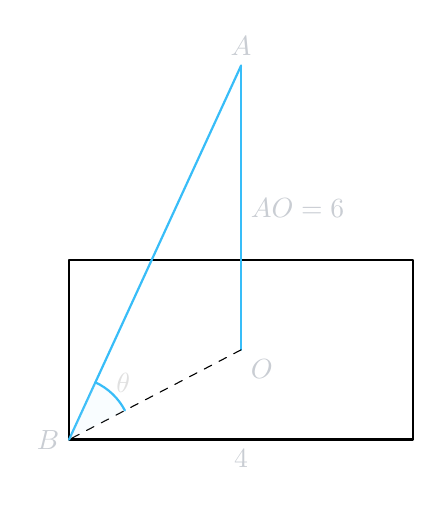
\begin{tikzpicture}[scale=0.95, line cap=round, line join=round]
  \coordinate (O) at (0,0);
  \coordinate (B) at (-2.3,-1.2);
  \coordinate (E) at (2.3,-1.2);
  \coordinate (D) at (2.3,1.2);
  \coordinate (C) at (-2.3,1.2);
  \coordinate (A) at (0,3.8);

  \draw[thick] (B)--(E)--(D)--(C)--cycle;
  \draw[cyan, thick] (A)--(O);
  \draw[cyan, thick] (A)--(B);
  \draw[dashed] (O)--(B);

  \node[right] at (0,1.9) {\textcolor{muted}{$AO=6$}};

  % ALWAYS internal (non-reflex) angle
  \InternalAngle[IntAngle]{A}{B}{O}{\theta}

  \node[above] at (A) {\textcolor{muted}{$A$}};
  \node[left] at (B) {\textcolor{muted}{$B$}};
  \node[below right] at (O) {\textcolor{muted}{$O$}};
  \node[below] at ($(B)!0.5!(E)$) {\textcolor{muted}{$4$}};
\end{tikzpicture}
\end{center}

\tcblower
\textcolor{green}{\bfseries Answer:}
\[
\begin{aligned}
\Step{1}\;& \text{Base side }s=4\ \Rightarrow\ \text{base diagonal }=s\sqrt2=4\sqrt2.\\
\Step{2}\;& \text{Distance from centre to a vertex: }OB=\frac{4\sqrt2}{2}=2\sqrt2\ \text{cm}.\\
\Step{3}\;& \text{Angle between }AB\text{ and the base plane}=\angle ABO=\theta.\\
\Step{4}\;& \text{In right }\triangle AOB:\quad \tan\theta=\frac{AO}{OB}=\frac{6}{2\sqrt2}=\frac{3}{\sqrt2}.\\
\Step{5}\;& \theta=\tan^{-1}\!\left(\frac{3}{\sqrt2}\right)\approx 64.76^\circ.
\end{aligned}
\]
\[
\boxed{\text{Angle between }AB\text{ and plane }BCDE\ \approx\ 64.76^\circ.}
\]
\end{QAPair}

% ============================================================
% Q7
\begin{QAPair}{Question 7 (i) -- (iv)}
\textcolor{gold}{\bfseries Question:} A room is $9\text{ m}$ long and $6\text{ m}$ wide. The angle of elevation from the bottom left corner to the top right corner is $49^\circ$.\\
(i) Find the floor diagonal.\\
(ii) Find the height of the room.\\
(iii) Find the angle of elevation from the bottom corner of the $9\text{ m}$ wall to the opposite top corner of that wall.\\
(iv) Find the angle of depression from the top corner of the $6\text{ m}$ wall to the opposite bottom corner of that wall.\\[6pt]

\begin{center}
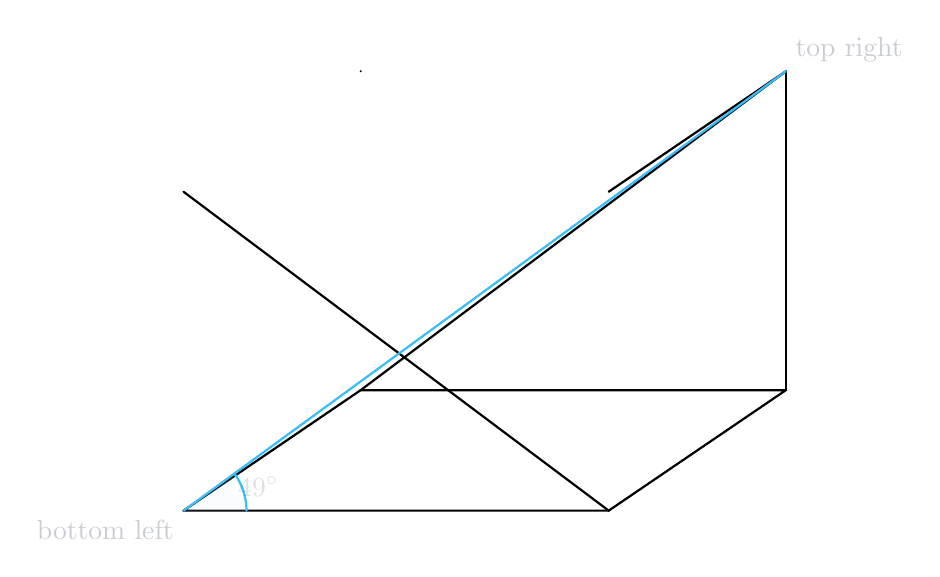
\begin{tikzpicture}[scale=0.9, line cap=round, line join=round]
  % floor rectangle and space diagonal schematic
  \coordinate (P) at (0,0);      % bottom-left
  \coordinate (Q) at (6,0);      % along 9m (scaled)
  \coordinate (R) at (8.5,1.7);  % depth (scaled)
  \coordinate (S) at (2.5,1.7);

  \coordinate (T) at (8.5,6.2);  % top-right
  \draw[thick] (P)--(Q)--(R)--(S)--cycle;       % floor
  \draw[thick] (S)--(S)+(0,4.5);
  \draw[thick] (R)--(T);
  \draw[thick] (Q)--(Q)+(0,4.5);
  \draw[thick] (P)--(P)+(0,4.5);
  \draw[thick] (P)+(0,4.5)--(Q)+(0,4.5)--(T)--(S)+(0,4.5)--cycle;

  \draw[cyan, thick] (P)--(T);   % space diagonal

  % ALWAYS internal (non-reflex) angle
  \InternalAngle[IntAngle]{Q}{P}{T}{49^\circ}

  \node[below left] at (P) {\textcolor{muted}{bottom left}};
  \node[above right] at (T) {\textcolor{muted}{top right}};
\end{tikzpicture}
\end{center}

\tcblower
\textcolor{green}{\bfseries Answer:}
\[
\begin{aligned}
\Step{1}\;& \text{(i) Floor diagonal }d=\sqrt{9^2+6^2}=\sqrt{81+36}=\sqrt{117}\approx 10.82\ \text{m}.\\[4pt]
\Step{2}\;& \text{(ii) Using }\tan 49^\circ=\frac{h}{d}\Rightarrow h=d\tan 49^\circ\\
&\Rightarrow h=\sqrt{117}\tan 49^\circ\approx 10.82(1.1504)\approx 12.44\ \text{m}.\\[4pt]
\Step{3}\;& \text{(iii) On the }9\text{ m wall: }\ \tan\alpha=\frac{h}{9}\Rightarrow \alpha=\tan^{-1}\!\left(\frac{12.44}{9}\right)\approx 54.10^\circ.\\[4pt]
\Step{4}\;& \text{(iv) On the }6\text{ m wall: }\ \tan\beta=\frac{h}{6}\Rightarrow \beta=\tan^{-1}\!\left(\frac{12.44}{6}\right)\approx 64.24^\circ.\\
&\text{(Angle of depression equals the corresponding angle of elevation.)}
\end{aligned}
\]
\[
\boxed{
\begin{aligned}
&\text{(i) }d\approx 10.82\text{ m},\quad
\text{(ii) }h\approx 12.44\text{ m},\\
&\text{(iii) }\alpha\approx 54.10^\circ,\quad
\text{(iv) }\beta\approx 64.24^\circ.
\end{aligned}}
\]
\end{QAPair}

% ============================================================
% Q8
\begin{QAPair}{Question 8 (i) -- (iii)}
\textcolor{gold}{\bfseries Question:} Three satellites $A,B,C$ are in the same plane. The distance $AB=15\text{ km}$. If $D$ is a house such that $\angle BAD=70^\circ$ and $ACBD$ is a rhombus, then: \\
(i) find $AC$, \quad (ii) find $BC$, \quad (iii) find $CD$ (distance from satellite $C$ to house $D$).\\[6pt]

\begin{center}
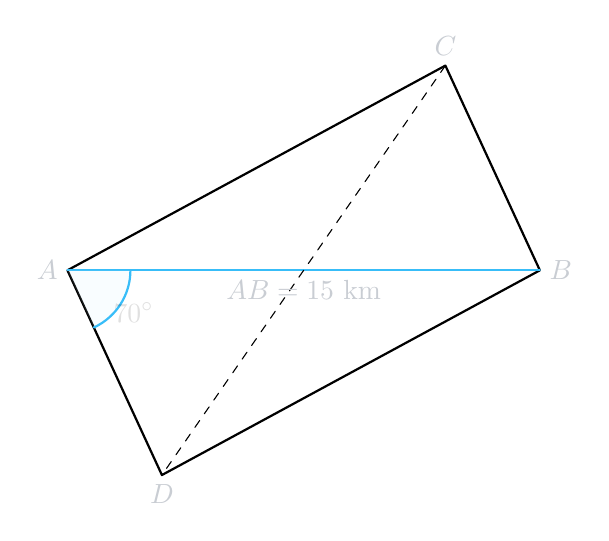
\begin{tikzpicture}[scale=1.0, line cap=round, line join=round]
  \coordinate (A) at (0,0);
  \coordinate (B) at (6,0);
  \coordinate (D) at (1.2,-2.6);
  \coordinate (C) at (4.8,2.6);

  \draw[thick] (A)--(C)--(B)--(D)--cycle;
  \draw[cyan, thick] (A)--(B); % diagonal AB
  \draw[dashed] (C)--(D);      % other diagonal CD

  % ALWAYS internal (non-reflex) angle
  \InternalAngle[IntAngle]{B}{A}{D}{70^\circ}

  \node[left] at (A) {\textcolor{muted}{$A$}};
  \node[right] at (B) {\textcolor{muted}{$B$}};
  \node[above] at (C) {\textcolor{muted}{$C$}};
  \node[below] at (D) {\textcolor{muted}{$D$}};
  \node[below] at ($(A)!0.5!(B)$) {\textcolor{muted}{$AB=15$ km}};
\end{tikzpicture}
\end{center}

\tcblower
\textcolor{green}{\bfseries Answer:}
\[
\begin{aligned}
\Step{1}\;& ACBD\text{ is a rhombus }\Rightarrow AC=CB=BD=DA=s\ (\text{say}).\\
\Step{2}\;& \text{In a rhombus, diagonal }AB\text{ bisects angle at }A.\\
&\Rightarrow \angle CAB=\angle BAD=70^\circ \ \text{and hence }\angle CAD=140^\circ.\\
\Step{3}\;& \text{Consider }\triangle ADB:\ AD=DB=s\text{ and }AB=15.\\
&\angle DAB=70^\circ,\ \angle DBA=70^\circ \Rightarrow \angle ADB=40^\circ.\\
\Step{4}\;& \text{Sine rule in }\triangle ADB:\\
&\frac{AB}{\sin 40^\circ}=\frac{s}{\sin 70^\circ}
\Rightarrow s=15\cdot\frac{\sin 70^\circ}{\sin 40^\circ}\approx 21.93\ \text{km}.\\
\Step{5}\;& \text{(i) }AC=s\approx 21.93\ \text{km},\qquad \text{(ii) }BC=s\approx 21.93\ \text{km}.\\
\Step{6}\;& \text{(iii) }CD\text{ is the other diagonal. In }\triangle ACD:\ CA=DA=s,\ \angle CAD=140^\circ.\\
&CD^2=s^2+s^2-2s^2\cos 140^\circ=2s^2(1-\cos 140^\circ)=2s^2(1+\cos 40^\circ).\\
&\Rightarrow CD=2s\cos 20^\circ\approx 2(21.93)\cos 20^\circ\approx 41.21\ \text{km}.
\end{aligned}
\]
\[
\boxed{
AC\approx 21.93\ \text{km},\quad
BC\approx 21.93\ \text{km},\quad
CD\approx 41.21\ \text{km}.}
\]
\end{QAPair}

\end{document}
